\newcommand{\binser}{Binary Search Tree \normalfont{\emoji{evergreen-tree}}}

\section{Optimal \binser}

In questo capitolo andremo a cercare un approccio di programmazione dinamica per
ottimizzare la ricerca in un \binser. Per rinfrescare la memoria faremo un breve
ripasso sui concetti chiave dei \binser.

\begin{figure}[H]
    \centering
    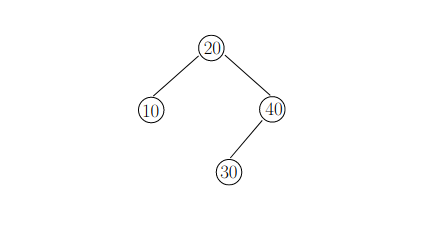
\includegraphics[width=10cm, keepaspectratio]{capitoli/dynamic_programming/imgs/binser.png}
    \caption{Esempio di un \binser.}
\end{figure}

Un \binser $T$ è una struttura dati che salva gli elementi secondo la
seguente proprietà: considerando che, in ogni nodo viene salvata una chiava (un
intero), la chiave di un nodo $u$ è più grande di ogni chiave del suo
sotto-albero sinistro e più piccola di ogni chiave del suo sotto-albero destro.\\
Inoltre, diamo le seguenti definizioni:

\begin{itemize}
    \item \textbf{livello}: il livello di un nodo $u$ è il numero di archi che si trovano tra la radice e $u$ stesso (il livello della radice è 0). Si denota con $level_T(u)$ .
    \item \textbf{profondità}: è il livello massimo dell'albero.
    \item \textbf{costo di ricerca}: il costo di ricerca per un nodo $u$ è proporzionale a $1 + level_T(u)$ .
    \item \textbf{bilanciato}: un albero è bilanciato se ha profondità uguale a $O(log n)$ .
\end{itemize}

L'essere bilanciato è una proprietà buona se ogni nodo viene cercato con la
stessa probabilità, ma dato che non è sempre così, possiamo cercare degli
algoritmi che vanno ad ottimizzare i casi in cui le probabilità siano
differenti.\\

Per cominciare a pensare ad un approccio di ottimizzazione possiamo provare a
tenere in considerazione il costo medio di ricerca di un nodo ($avgcost(T)$)
rispetto alla probabilità che esso venga ricercato ($freq(k)$) e al suo costo
di ricerca ($cost(k)$).

\[
    avgcost(T) = \sum_{i=1}^{n} freq(k_i) \cdot cost(k_i)
\]

\subsection{Il Problema}

Più formalmente definiamo il problema come segue:

\begin{boxed}
    Dato in input:
    \begin{itemize}
        \item un insieme $S$ di $n$ interi
        \item un array $W$ dove $W[i] (1 \leq i \leq n)$ contiene un peso intero positivo
    \end{itemize}

    vogliamo trovare un Bin Ser Tree $T$ su $S$ che ha costo medio \textit{minimo}.

    \[
        avgcost(T) = \sum_{i=1}^{n} W[i] \cdot cost_T(i)
    \]

    dove $cost_T(i) = 1 + level_T(i)$ , ovvero il numero di nodi a cui si accede per trovare
    la chiave $i$ in $T$ .
\end{boxed}

Questa definizione può essere generalizzata spostando il nodo di partenza dalla
radice ad un nodo qualsiasi come segue:

\begin{boxed}
    Dato in input:
    \begin{itemize}[itemsep=0.5pt]
        \item un insieme $S$ di $n$ interi
        \item un array $W$ dove $W[i] (1 \leq i \leq n)$ contiene un peso intero
              positivo
        \item due interi $a, b$ che soddisfano $(1 \leq a \leq b \leq n)$
    \end{itemize}

    vogliamo trovare un Bin Ser Tree $T$ su $\{a, a+1, \ldots, b\}$ che ha costo
    medio \textit{minimo}.

    $$avgcost(T) = \sum_{i=a}^{b} W[i] * cost_T(i)$$

    dove $cost_T(i) = 1 + level_T(i)$ , ovvero il numero di nodi a cui si accede
    per trovare la chiave $i$ in $T$ .
\end{boxed}

\subsection{Funzionamento}

Per spiegare la costruzione di questo algoritmo andremo a dividerlo in 3 passi:

\begin{itemize}
    \item Identificare tutti i possibili step iniziali
    \item In base allo step iniziale, trovare la soluzione ottima
    \item Trovare quale step iniziale porta alla miglior soluzione possibile
\end{itemize}

\paragraph{Step 1:}
In questo step cercheremo la radice dell'albero che una volta trovata ci andrà a
dividere i due sotto-alberi. Formalmente, supponiamo di definire $r$ come chiave
della radice, allora il sotto-albero sinistro $T_1$ deve essere definito su $S_1
    = \{a, \ldots, r -1\}$ e il sotto-albero destro $T_2$ deve essere definito su
$S_2 = \{r + 1, \ldots, b\}$.

\begin{figure}[H]
    \centering
    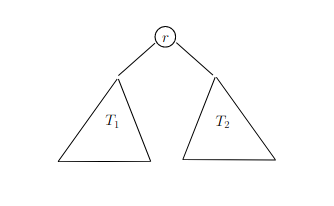
\includegraphics[width=10cm, keepaspectratio]{capitoli/dynamic_programming/imgs/binser_subtree.png}
    \caption{La figura mostra la scelta della radice e la relativa suddivisione dei due sotto-alberi.}
\end{figure}

\paragraph{Step 2:}
Scelta $r$ come radice, dobbiamo ora cercare i migliori sotto-alberi $T_1$ e
$T_2$ per minimizzare il costo medio di $T$. Per farlo scomponiamo la definizione
data in precedenza di $avgcost(T)$ affinché possa avanzare ricorsivamente
all'interno dei due sotto-alberi. Otteniamo quindi la seguente funzione:

\[
    avgcost(T) = (\sum_{i=a}^b W[i]) + avgcost(T_1) + avgcost(T_2)
\]

Intuitivamente dobbiamo minimizzare $avgcost(T_1)$ e $avgcost(T_2)$.\\

La definizione appena data non è implementativamente corretta, quindi definiamo
una versione più chiara ed utilizzabile:

\begin{boxed}
    Definiamo $optavg(a,b)$ come:

    \begin{itemize}[itemsep=0.5pt]
        \item $0$ se $a > b$
        \item il Binary Search Tree di costo medio minore su $\{a, a+1, \ldots, b\}$ , altrimenti
    \end{itemize}

    Il costo medio ottimo è definito da $optavg(a, b | r)$ che è uguale a:

    \[
        (\sum_{i=a}^b W[i]) + optavg(a, r-1) + optavg(r+1, b)
    \]

\end{boxed}

\paragraph{Step 3:}
Questa è la soluzione ottima per una data radice $r$ e visto che noi dobbiamo
cercarla per tutte le possibili combinazioni di $r$, possiamo riscrivere
$optavg$ come segue:

\[
    optavg(a, b) = \min_{r=a}^b optavg(a, b | r) = (\sum_{i=a}^b W[i]) +  \min_{r=a}^b \{optavg(a, r-1) + optavg(r+1, b)\}
\]

Questa è la struttura ricorsiva del problema.

\paragraph{Riassumendo:}
dato un array $W$ di $n$ interi il \binser ottimo è dato dalla seguente
ricorsione:

% TODO: fix this
% \[
%     optavg(a, b) =
%     \begin{cases}
%         0 & if a > b \\
%         %(\sum_{i=a}^b W[i]) + \min_{r=a}^b \{optavg(a, r-1) + optavg(r +1, b)\} & \text{otherwise}
%     \end{cases}
% \]

Il costo temporale per calcolare $optavg(1,n)$ è uguale a $O(n^3)$, questo
ovviamente ci restituisce solamente il costo, per poterci costruire l'albero
possiamo recuperare le informazioni in $O(n)$.